% Commenti speciali

% !TEX encoding = UTF-8 Unicode
% !TEX TS-program = pdflatex
% !TEX spellcheck = it-IT
% !TEX root = Dispensa/afed.tex

% Capitolo 4
\chapter{Alcuni complementi di calcolo delle variazioni}\label{Alcuni complementi di calcolo delle variazioni}
Benvenuti nel magico mondo del Calcolo delle Variazioni! Prima di proseguire si consiglia la lettura di
\begin{center}
	\href{https://www.dmf.unicatt.it/~musesti/FM/}{FISICA MATEMATICA\\
		appunti a cura di Alessandro Musesti}
\end{center}
non ve ne pentirete! :-)

Nel seguito, salvo diversa specificazione, $U$ indicherà un generico sottoinsieme aperto limitato di $\R^n$ con $\partial U$ di classe $C^1$. 
\section{Variazione prima e variazione seconda}
\begin{definizione}
	Chiamiamo \emph{lagrangiana}\index[analitico]{lagrangiana} ogni applicazione $L: \overline{U} \times \R \times \R^n \to \R$ di classe $C^\infty$ tale che
	\[ L(x,s,\xi) = L(x_1,\dots,x_n, s, \xi_1,\dots,\xi_n) \]
\end{definizione}
Nel seguito considereremo funzionali della forma
\[ I[u] = \int_U L(x,u(x),Du(x))d\mathcal{L}^n(x) \]
definiti inizialmente per $u \in C^\infty(\overline{U})$ tali che $u= g \textup{ su } \partial U,$ con $g$ un'applicazione nota. Il funzionale $I$ è anche detto \emph{energia} in quanto molto spesso può essere interpretato come energia meccanica di un particolare sistema fisico.
\begin{definizione}
	Sia $v \in C^\infty_c(U)$. Consideriamo l'applicazione $i: \R \to \R$ tale che
	\[  i(\tau) = I[u+\tau v].\]
	Chiamiamo \emph{variazione prima}\index[analitico]{variazione!prima} di $I$ la derivata prima di $i$, $i'(\tau)$, e \emph{variazione seconda}\index[analitico]{variazione!seconda} di $I$ la derivata seconda di $i$, $i''(\tau)$.
\end{definizione}
\begin{proposizione}\emph{\textbf{(condizioni necessarie per l'esistenza di minimi)}}
	Se $I$ ammette minimo in $u$, allora $i$ ammette minimo in $0$. In particolare, 
	\begin{align*}
		i'(0) &= 0, & i''(0)\ge 0.
	\end{align*}
	
	\begin{proof}
		Innanzitutto, per ogni $v \in C^\infty_c(U), \tau \in \R$, 
		\[ u + \tau v = g \textup{ su } \partial U \]
		in quanto $I$ ammette minimo in $u$. Allora, per ogni $v \in C^\infty_c(U), \tau \in \R$
		\[ I[u] \le I[u + \tau v] \]
		ossia $i(0) \le i(\tau)$ per ogni $\tau \in \R$, da cui la tesi.
	\end{proof}
\end{proposizione}
Calcoliamo esplicitamente in queste iniziali condizioni di regolarità la variazione prima di $I$ in un suo minimo $u$. 

Mostriamo innanzitutto che l'applicazione $f: \R \times \overline{U} \to \R $ tale che
\[ f(\tau, x) = L(x,u(x)+\tau v(x),Du(x)+\tau Dv(x)) \]
soddisfa le ipotesi del Teorema di derivazione sotto il segno di integrale. Innanzitutto, per ogni $\tau \in \R$, essendo $L$ di classe $C^\infty$, $u \in C^\infty(\overline{U})$ e $v \in C^\infty_c(U)$, allora sicuramente l'applicazione ${x \mapsto f(\tau,x)}$ è almeno continua in $\overline{U}$. In particolare è sommabile. Poi per ogni $x \in \overline{U}$, sempre per il fatto che $L$ è di classe $C^\infty$, allora l'applicazione ${\tau \mapsto f(\tau,x)}$ è derivabile. Ora,
\begin{align*}
	\frac{\partial f}{\partial \tau}(\tau,x) &= D_sL(x,u(x)+\tau v(x),Du(x)+ \tau Dv(x))v(x) + \\
	&+D_{\xi}L(x,u(x)+\tau v(x),Du(x)+\tau Dv(x))\cdot Dv(x)
\end{align*}
e non essendo restrittivo supporre $\tau \in [-1,1]$ si ha 
\[ \abs*{\frac{\partial f}{\partial \tau}(\tau,x)} \le A\norm{Dv}_\infty + B\norm{v}_\infty \]
dove 
\[ A = \max\Set{\abs{D_\xi L(x,s,\xi)} : \abs{\xi} \le \norm{Du}_\infty + \norm{Dv}_\infty, \abs{s} \le \norm{u}_\infty + \norm{v}_\infty, x \in \overline{U}} \]
e 
\[ B = \max\Set{\abs{D_s L(x,s,\xi)} : \abs{\xi} \le \norm{Du}_\infty + \norm{Dv}_\infty, \abs{s} \le \norm{u}_\infty + \norm{v}_\infty, x \in \overline{U}}. \]
Allora, detto $g = \left( A\norm{Dv}_\infty + B\norm{v}_\infty\right)\chi_{\overline{U}} : \overline{U} \to \R$, si ha per ogni $x \in \overline{U}$
\[ \abs*{\frac{\partial f}{\partial \tau}(\tau,x)} \le g(x) \]
con $g$ sommabile. 

Per il Teorema di derivazione sotto il segno di integrale quindi 
\begin{align*}
	i'(\tau) &=\int_U \Bigl( D_sL(x,u(x)+\tau v(x),Du(x)+\tau Dv(x))v(x) + \\
	& + D_{\xi}L(x,u(x)+\tau v(x),Du(x)+\tau Dv(x))\cdot Dv(x)\Bigr) d\mathcal{L}^n(x) 
\end{align*}
e posto $\tau = 0$ otteniamo 
\[ \int_U \Bigl( D_sL(x,u(x),Du(x))v(x) + D_{\xi}L(x,u(x),Du(x))\cdot Dv(x)\Bigr) d\mathcal{L}^n(x) = 0. \]
A questo punto, siccome $v$ ha supporto compatto, per la formula di Gauss--Green
\[ \int_U \Bigl( D_sL(x,u(x),Du(x)) -\sum_{i=1}^{n} D_{x_i}\bigl( D_{\xi_i}L(x,u(x),Du(x))\bigr) \Bigr)v(x) d\mathcal{L}^n(x) = 0 \]
ed il Lemma di Du Bois--Reymond si conclude che 
\[  D_sL(x,u(x),Du(x)) -\sum_{i=1}^{n} D_{x_i}\bigl( D_{\xi_i}L(x,u(x),Du(x))\bigr) = 0 \textup{ in } U. \]
\begin{definizione}
	Chiamiamo \emph{equazione di Eulero--Lagrange}\index[analitico]{equazione!di Eulero--Lagrange} associata al funzionale $I$, l'equazione differenziale alle derivate parziali quasilineare del secondo ordine in forma di divergenza
	\[ -\sum_{i=1}^{n} D_{x_i}\bigl( D_{\xi_i}L(x,u(x),Du(x))\bigr)  + D_sL(x,u(x),Du(x)) = 0. \]
\end{definizione}
Se $u$ è un minimo di $I$, allora risolve l'equazione di Eulero--Lagrange associata ad $I$. Molto spesso, si cerca proprio di ricondurre una PDE ad un funzionale in quanto è solitamente estremamente più semplice trovare i punti critici di un funzionale rispetto che risolvere direttamente l'equazione.
\begin{esempio}
	Consideriamo
	\[ L(x,s,\xi) = \frac{1}{2}\sum_{i,j=1}^{n}a_{ij}(x)\xi_i\xi_j - sf(x) \]
	con $a_{ij}(x) = a_{ji}(x)$ per ogni $i,j=1,\dots,n$. Allora, siccome per ogni $i,j=1,\dots,n$
	\begin{align*}
		D_{\xi_i} L &= \sum_{j=1}^n a_{ij}\xi_j, & D_s L = -f,
	\end{align*}
	l'equazione di Eulero--Lagrange associata al funzionale 
	\[ I[u] = \int_U  \left( \frac{1}{2}\sum_{i,j=1}^{n}a_{ij}(x)\xi_i\xi_j - sf(x)\right) d\mathcal{L}^n(x)\]
	è 
	\[ -\sum_{i,j=1}^n D_{x_i}\left( a_{ij}(x)D_{x_j}u(x)\right)  = f(x) \textup{ in } U, \]
	ossia un'equazione alle derivate parziali lineare del secondo ordine in forma di divergenza.
\end{esempio}

Non è detto, almeno a priori, che un minimo sia una soluzione in senso classico.
\begin{esempio}
	Consideriamo il problema
	\[ 	\begin{cases}
		-\Delta u = 0 & \textup{in } U,\\
		u= g & \textup{su } \partial U.
	\end{cases} \]
	Il funzionale associato è 
	\[ I[u] = \frac{1}{2}\int_U \abs{Du}^2 d\mathcal{L}^n. \]
	Se fossimo alla ricerca di soluzioni classiche, dovremmo cercare di dimostrare l'esistenza di minimi per $I$ su
	\[ C^2_g(U) = \left\lbrace u \in C^2(U) \cap C(\overline{U}): u = g \textup{ su } \partial U\right\rbrace. \]
	Provando ad applicare il Metodo diretto, prendiamo $(u_h)$ in $C^2_g(U)$ tale che 
	\[ I[u_h] \le \underset{u \in  C^2_g(U)}{\min}\;I[u] + \frac{1}{h+1}. \]
	Per andare avanti avremmo bisogno di un risultato di compattezza, tuttavia nel dominio dove stiamo lavorando non lo abbiamo. Possiamo esibire il seguente controesempio: siano $U = \left] -1,1\right[ $, $g = 1$ e 
	\[ u_h(x) = \sqrt{\frac{1}{h} +x^2} - \left( \sqrt{\frac{1}{h} +1}-1\right).  \]
	Chiaramente $u_h$ è di classe $C^\infty$ per ogni $h \in \N$. Inoltre,
	\[ I[u_h] = \frac{1}{2}\int_{-1}^{1} \frac{x^2}{\left( \frac{1}{h}+x^2\right) }dx \le \frac{1}{2} \int_{-1}^{1}dx = 1 < +\infty. \]
	Eppure, detto $\overline{u}(x) = \abs{x}$, da due razionalizzazioni inverse emerge che
	\[ \abs{u_h(x) - \overline{u}(x)} = \abs*{\left( \sqrt{ \frac{1}{h} + x^2} - \sqrt{x^2}\right) + \left( 1-  \sqrt{ \frac{1}{h} + 1}\right) }\le \frac{2}{\sqrt{h}}, \]
	quindi $u_h \to \overline{u}$ uniformemente, ma $\overline{u} \notin C^2_g(U)$.
\end{esempio}
\begin{esempio}\textbf{\emph{(superfici minime)}}
	Consideriamo il funzionale d'area 
	\[ I[u] = \int_U \sqrt{1 + \abs{Du}^2}d\mathcal{L}^n. \]
	L'equazione di Eulero--Lagrange associata è 
	\[ \sum_{i=1}^nD_{x_i}\left( \frac{D_{x_i} u}{\sqrt{1 + \abs{Du}^2}}\right)  = 0 \textup{ in } U \]
	ed è detta \emph{equazione delle superfici minime}. L'espressione a primo membro è $n$ volte la curvatura media del grafico di $u$, quindi le superfici minime sono caratterizzate da curvatura media nulla.
\end{esempio}

Calcoliamo esplicitamente in queste iniziali condizioni di regolarità anche la variazione seconda di $I$ in un suo minimo $u$. In modo analogo a quanto fatto per il calcolo della variazione prima, si verifica che è applicabile il Teorema di derivazione sotto il segno di integrale, quindi 
\begin{align*}
	i''(\tau) &= \int_U \Biggl( \sum_{i,j=1}^nD^2_{\xi_i,\xi_j}L(x,u(x)+\tau v(x), Du(x)+\tau Dv(x)) D_{x_i}v(x)D_{x_j}v(x) +  \\
	&+  2 \sum_{i=1}^nD^2_{\xi_i,s}L(x,u(x)+\tau v(x), Du(x)+\tau Dv(x)) D_{x_i} v(x) v(x) + \\
	&+ D^2_{s,s} L(x,u(x)+\tau v(x), Du(x)+\tau Dv(x)) v(x)^2\Biggr) d\mathcal{L}^n(x)
\end{align*}
e posto $\tau = 0$ si ha
\begin{align*}
	\int_U \Biggl( &\sum_{i,j=1}^nD^2_{\xi_i,\xi_j}L(x,u(x), Du(x)) D_{x_i}v(x)D_{x_j}v(x) + \\
	&+2 \sum_{i=1}^nD^2_{\xi_i,s}L(x,u(x), Du(x)) D_{x_i} v(x) v(x) + \\
	&+ D^2_{s,s} L(x,u(x), Du(x)) v(x)^2\Biggr) d\mathcal{L}^n(x) \ge 0
\end{align*}
per ogni $v \in C^\infty_c(U)$.

Cerchiamo di estrarre delle informazioni dalla disuguaglianza precedente. Innanzitutto, mediante approssimazione è possibile dimostrare la validità della disuguaglianza per $v$ lipschitziane che si annullano su $\partial U$. 

Consideriamo ora  $\varrho : \R \to \R$ l'applicazione tale che per ogni $x \in \R$ 
\[ \varrho(x+1) = \varrho(x) \]
e 
\[  \varrho(x) = \begin{cases}
	x & \textup{se } 0\le x \le \frac{1}{2}, \\
	1-x & \textup{se } \frac{1}{2}\le x \le 1. \\
\end{cases} \]
Evidentemente $\abs{\varrho'} = 1 $ q.o. in $\R$. Ora, dati $\varepsilon>0, \eta \in \R^n $, $\zeta \in C^\infty_c(U)$ definiamo per ogni $x \in U$
\[ v(x) = \varepsilon \varrho\left( \frac{x\cdot \eta}{\varepsilon}\right) \zeta(x) \]
e osserviamo che 
\[ D_{x_i} v(x) = \varrho'\left( \frac{x\cdot \eta}{\varepsilon}\right) \eta_i \zeta(x) + \varepsilon \varrho\left( \frac{x\cdot \eta}{\varepsilon}\right)  D_{x_i} \zeta(x). \]
Pertanto,
\[ 0 \le \int_U  \sum_{i,j=1}^n D^2_{\xi_i,\xi_j}L(x,u(x), Du(x)) \varrho'(x)^2\eta_i\eta_j \zeta(x)^2 d\mathcal{L}^n(x) + C_1 \varepsilon + C_2 \varepsilon^2  \]
e, se $\varepsilon \to 0^+$, ricordando che $\abs{\varrho'} = 1 $ q.o. in $\R$,
\[ 0 \le \int_U \sum_{i,j=1}^n D^2_{\xi_i,\xi_j}L(x,u(x), Du(x))\eta_i\eta_j \zeta(x)^2 d\mathcal{L}^n(x). \]
In definitiva\footnote{Si tratta di applicare una versione del Lemma di Du Bois--Reymond per le disuguaglianze.}, per ogni $\eta \in \R^n$ e per ogni $x \in U$
\[ \sum_{i,j=1}^n D^2_{\xi_i,\xi_j}L(x,u(x), Du(x))\eta_i\eta_j \ge 0,\]
da cui capiamo che sarà naturale supporre, nella prossima sezione, che $L$ sia convesso nei gradienti.

Prima di procedere, però, vediamo alcuni accenni al caso vettoriale.
\begin{definizione}
	Chiamiamo \emph{lagrangiana}\index[analitico]{lagrangiana} ogni applicazione $L: \overline{U} \times \R^m \times \textup{Mat}_{m,n}(\R) \to \R$ di classe $C^\infty$ tale che
	\[ L(x,s,\xi) = L(x_1,\dots, x_j,\dots,x_n, s_1,\dots,s_i,\dots,s_m, \xi_{11},\dots,\xi_{ij},\dots,\xi_{mn}) \]
\end{definizione}
Si considerano funzionali della forma
\[ I[u] = \int_U L(x,u(x),Du(x))d\mathcal{L}^n(x) \]
definiti per $u \in C^\infty(\overline{U};\R^m)$ tali che $u= g \textup{ su } \partial U,$ con $g: \partial U \to \R^m$ un'applicazione nota. Come nel caso scalare, il funzionale $I$ è anche detto \emph{energia} in quanto molto spesso può essere interpretato come energia meccanica di un particolare sistema fisico.
\begin{definizione}
	Sia $v \in C^\infty_c(U;\R^m)$. Consideriamo l'applicazione $i: \R \to \R$ tale che
	\[  i(\tau) = I[u+\tau v].\]
	Chiamiamo \emph{variazione prima}\index[analitico]{variazione!prima} di $I$ la derivata prima di $i$, $i'(\tau)$, e \emph{variazione seconda}\index[analitico]{variazione!seconda} di $I$ la derivata seconda di $i$, $i''(\tau)$.
\end{definizione}
\begin{proposizione}\emph{\textbf{(condizioni necessarie per l'esistenza di minimi)}}
	Se $I$ ammette minimo in $u$, allora $i$ ammette minimo in $0$. In particolare, 
	\begin{align*}
		i'(0) &= 0, & i''(0)\ge 0.
	\end{align*}
	
	\begin{proof}
		Si tratta di una semplice variante del caso scalare.
	\end{proof}
\end{proposizione}
In modo analogo a quanto fatto per il caso scalare, possiamo calcolare esplicitamente la variazione prima di $I$ in un suo minimo $u$. Da questo calcolo emerge, in tutta analogia, la seguente definizione.
\begin{definizione}
	Chiamiamo \emph{(sistema di) equazioni di Eulero--Lagrange}\index[analitico]{equazione!di Eulero--Lagrange} associate al funzionale $I$, il sistema di equazioni differenziali alle derivate parziali quasilineari del secondo ordine in forma di divergenza
	\[ \begin{cases}
		D_{s_1}L(x,u(x),Du(x))-\displaystyle \sum_{i=j}^{n} D_{x_j}\bigl( D_{\xi_{1j}}L(x,u(x),Du(x))\bigr) = 0 & \textup{in } U,\\
		& \vdots,\\
		D_{s_m}L(x,u(x),Du(x))-\displaystyle\sum_{j=1}^{n} D_{x_j}\bigl( D_{\xi_{mj}}L(x,u(x),Du(x))\bigr) = 0 & \textup{in } U.
	\end{cases}\]
\end{definizione}

\begin{definizione}
	Diciamo che $L$ è una \emph{lagrangiana nulla}\index[analitico]{lagrangiana!nulla} se ogni $u \in C^2(\overline{U};\R^m)$ è soluzione delle equazioni di Eulero--Lagrange.
\end{definizione}

\begin{teorema}
	Sia $L$ una lagrangiana nulla. Se $u,\overline{u}\in C^2(\overline{U};\R^m)$ tali che $u = \overline{u}$ su $\partial U$, allora $I[u] = I[\overline{u}]$.
\end{teorema}
\begin{proof}
	Consideriamo l'applicazione $j: [0,1] \to \R$ tale che	
	\[ j(\tau) = I[\tau u + (1-\tau)\overline{u}]. \]
	Allora, in modo analogo a quanto visto per il calcolo della variazione prima nel caso scalare, 
	\begin{align*}
		&j'(\tau) = \int_U \left( \sum_{i=1}^{m}D_{s_i}L(x,\tau u(x)+(1-\tau)\overline{u}(x), \tau Du(x) + (1-\tau)D\overline{u}(x))(u_i(x)-\overline{u}_i(x)) + \right. \\
		&\left. \hspace{-5pt}+ \hspace{-2pt}\sum_{j=1}^{n} \sum_{i=1}^{m} \hspace{-2pt} D_{\xi_{ij}}L(x,\tau u(x)\hspace{-2pt}+\hspace{-2pt}(1-\tau)\overline{u}(x), \tau Du(x)\hspace{-2pt} + \hspace{-2pt}(1-\tau)D\overline{u}(x)) D_{x_j}(u_i(x)-\overline{u}_i(x))\hspace{-2pt} \right) \hspace{-4pt}d\mathcal{L}^n(x)
	\end{align*}
	e, combinando il fatto che $u - \overline{u} = 0$ su $\partial U$ con le formule di Gauss--Green,
	\begin{align*}
		&j'(\tau) = \sum_{i=1}^{m}\int_U \biggl( D_{s_i}L(x,\tau u(x)+(1-\tau)\overline{u}(x), \tau Du(x) + (1-\tau)D\overline{u}(x)) + \\
		&\left.\hspace{-2pt} - \hspace{-2pt}\sum_{j=1}^{n}\hspace{-2pt}D_{x_j}\hspace{-2pt}\left( \hspace{-2pt} D_{\xi_{ij}}L(x,\tau u(x)+(1-\tau)\overline{u}(x), \tau Du(x) + (1-\tau)D\overline{u}(x))\hspace{-2pt}\right)  \right)\hspace{-3pt}(u_i(x)-\overline{u}_i(x)) \hspace{-1pt}d\mathcal{L}^n(x)
	\end{align*}
	Siccome $\tau u +(1-\tau)\overline{u} \in C^2(\overline{U};\R^m)$ e $L$ una lagrangiana nulla, segue che $j'(\tau) = 0$ per ogni $\tau \in [0,1]$. In particolare, $j$ è costante su $[0,1]$, da cui $I[u] = j(1) = j(0) = I[\overline{u}]$, ossia la tesi.
\end{proof}

Se $m=1$, ossia nel caso scalare, le uniche lagrangiane nulle sono le funzioni lineari in $\xi$. 

\begin{definizione}
	Sia $A \in \textup{Mat}_{n}(\R)$. Chiamiamo \emph{matrice dei cofattori} di $A$\index[analitico]{matrice!dei cofattori}\index[simboli]{$\textup{cof}(A)$} la matrice 
	\[ \textup{cof}A \]
	dove $\textup{cof}(A)_{ij} = (-1)^{i+j}\det(A^{(ij)})$ e $A^{(ij)} \in \textup{Mat}_{n-1}(\R)$ è ottenuta da $A$ eliminando la $i$-esima riga e la $j$-esima colonna.
\end{definizione}
\begin{lemma}
	Se $u:\R^n \to \R^n$ di classe $C^2$, allora per ogni $i=1,\dots, n$
	\[ \sum_{j=1}^{n} D_{x_j}(\textup{cof}(Du)_{ij}) = 0,\]
	ossia, in forma vettoriale, $\div (\textup{cof}(Du)) = 0$.
\end{lemma}
\begin{proof}
	Innanzitutto, per ogni $\xi \in \textup{Mat}_{n}(\R)$
	\[ (\det \xi)\textup{Id} = \xi^T\textup{cof}(\xi), \]
	ossia per ogni $i,j=1,\dots,n$
	\begin{equation}\label{serve}
		(\det \xi)\delta_{ij} = \sum_{k=1}^{n} \xi_{ki}\textup{cof}(\xi)_{kj}.
	\end{equation}
	Scelto $\xi = Du$ in \eqref{serve}, deriviamo ambo i membri per $x_j$ e sommando su $j$ otteniamo per ogni $i=1,\dots, n$
	\[ \sum_{j,p,q=1}^{n} \delta_{ij}\textup{cof}(Du)_{pq}D^2_{x_j,x_q}u_p = \sum_{k,j=1}^{n}\left(  D^2_{x_j,x_i}u_k \textup{cof}(Du)_{kj} + D_{x_i}u_k D_{x_j}(\textup{cof}(Du)_{kj}) \right) \]
	che può essere riscritta, scambiando $q$ con $j$ e $p$ con $k$ a primo membro, come 
	\[ \sum_{k=1}^n D_{x_i}u_k \left( \sum_{j=1}^{n}D_{x_j}\textup{cof}((Du)_{kj})\right) =0, \]
	ossia come un sistema lineare omogeneo che, scambiando $k$ con $i$, è 
	\[ \sum_{i=1}^n D_{x_k}u_i \left( \sum_{j=1}^{n}D_{x_j}(\textup{cof}(Du)_{ij})\right) =0. \]
	
	A questo punto, se $\det Du(x_0) \ne 0$, il sistema ha solo la soluzione banale, ossia per ogni  $k=1,\dots,n$
	\[ \sum_{j=1}^{n}D_{x_j}(\textup{cof}(Du(x_0))_{kj})=0. \]
	Se, invece, $\det Du(x_0) = 0$, sia $\varepsilon >0$ tale che $\det(Du(x_0) + \varepsilon\textup{Id}) \ne 0$. Applicando quanto fatto sopra a $u + \varepsilon x$ e mandando poi $\varepsilon \to 0^+$ segue la tesi.
\end{proof}
\begin{teorema}
	L'applicazione 
	\[ L(\xi) = \det(\xi) \]
	è una lagrangiana nulla.
\end{teorema}
\begin{proof}
	Per \eqref{serve}, per ogni $i,j = 1,\dots,n$
	\[ D_{ \xi_{ij}} \det (\xi) = (\textup{cof}\xi)_{ij}, \]
	da cui per ogni $u \in C^2(\overline{U};\R^n)$ e per ogni $i =1,\dots,n$
	\[ \sum_{j=1}^n D_{x_j}\left( D_{\xi_{ij}}L(Du)\right) =0, \]
	che è la tesi.
\end{proof}
\begin{osservazione}
	Grazie al fatto che il determinante è una lagrangiana nulla, possiamo dare una dimostrazione alternativa del Teorema di Brouwer rispetto a quella riportata nel Capitolo \ref{Teoremi di punto fisso}. 
	
	Vediamo innanzitutto il caso $K = \overline{\B(0,1)}$. Mostriamo che non esiste alcuna applicazione $f: \overline{\B(0,1)} \to \partial \B(0,1)$ di classe $C^2$ tale che per ogni $x \in \partial \B(0,1)$ si abbia $f(x) = x$. Supponiamo, per assurdo, che una tale applicazione esista. Allora, siccome $\det$ è una lagrangiana nulla,
	\[ \int_{\B(0,1)} \det(Df) d\mathcal{L}^n = \int_{\B(0,1)} \det(Dx)d\mathcal{L}^n(x) = \int_{\B(0,1)}d\mathcal{L}^n = \mathcal{L}^n(\B(0,1)) \ne 0.\]
	D'altra parte, $f(x) \cdot f(x) = \abs{f(x)}^2 = 1$ per ogni $x \in \overline{\B(0,1)}$ quindi, differenziando ambo i membri,
	\[ (Df)^T f = 0. \]
	Allora, siccome $\abs{f} = 1$ su $\overline{\B(0,1)}$, $0$ è un autovalore per $(Df)^T$, quindi $\det(Df) = \det((Df)^T) = 0$, assurdo.
	
	Mostriamo quindi che non esiste alcuna applicazione $f: \overline{\B(0,1)} \to \partial \B(0,1)$ continua tale che per ogni $x \in \partial \B(0,1)$ si abbia $f(x) = x$. Supponiamo, per assurdo, che una tale applicazione esista. Estendiamo $f$ con continuità fuori da $ \overline{\B(0,1)}$ in modo che sui segmenti radiali assuma il valore che ha su $\partial \B(0,1)$. Chiaramente, $f$ è non nulla su tutto $\R^n$. Sia $\varepsilon >0$ tale che l'$\varepsilon$-mollificatore\footnote{Perché abbiamo bisogno di un'applicazione almeno di classe $C^2$, così è pure $C^\infty$.} $\varrho_\varepsilon$ realizzi $ \varrho_\varepsilon \ast f \ne 0$ su $\R^n$ e $\varrho_\varepsilon \ast f(x) = x$ su $\R^n\setminus{\B(0,2)}$. Detto ciò, l'applicazione $\frac{2\varrho_\varepsilon \ast f}{\abs{\varrho_\varepsilon \ast f}}$, a meno di un riscalamento, è un'applicazione liscia che è l'identità su $\partial \B(0,1)$, da cui l'assurdo.
	
	A questo punto, la conclusione segue in modo simile a come riportato nel Capitolo \ref{Teoremi di punto fisso}.
\end{osservazione}

\section{Esistenza ed unicità di minimi}
In questa sezione ci occupiamo del caso scalare. Nel seguito considereremo $q \in \left] 1,\infty\right[ $.

Se $L$ è coercitiva, esistono $\alpha>0,\beta \ge 0$ tali che per ogni $x \in U, s \in \R,\xi \in \R^n$
\[ L(x,s,\xi) \ge \alpha\abs{\xi}^q-\beta. \]
Allora, 
\[ I[u] = \int_U L(x,u,Du)d\mathcal{L}^n(x) \ge \int_U \left(\alpha\abs{Du}^q-\beta\right)d\mathcal{L}^n = \alpha \norm{Du}_{L^q(U)}^q -\gamma  \]
dove $\gamma = \beta \mathcal{L}^n(U) >0$. Riassumendo,
\begin{equation}
	I[u] \ge \alpha \norm{Du}_{L^q(U)}^q -\gamma,
\end{equation}
detta \emph{condizione di coercitività}\index[analitico]{condizione!di coercitività} di $I$. Osserviamo subito che se $\norm{Du}_{L^q(U)} \to +\infty,$ allora $I[u] \to +\infty$. La condizione di coercitività ha significato anche per $u$ meno regolari rispetto alle ipotesi iniziali. 

Non è detto, a priori, che il funzionale ammetta minimo.
\begin{esempio}
	Dato $ q \in \left] 2,2^\ast\right[$, sia $I: H^1_0(U) \to \R$ tale che 
	\[ I[u] = \frac{1}{2}\int_U \abs{Du}^2 d\mathcal{L}^n - \frac{1}{q}\int_U \abs{u}^q d\mathcal{L}^n. \]
	Dato $u_0 \in H^1_0(U)$, consideriamo la successione $(hu_0)$. Allora,
	\[ I[hu_0] = \frac{h^2}{2}\int_U \abs{Du}^2 d\mathcal{L}^n - \frac{h^q}{q}\int_U \abs{u}^q d\mathcal{L}^n \le C(h^2 - h^q) \to -\infty, \]
	quindi $I$ non può ammettere minimo su $H^1_0(U)$.
\end{esempio}
Considereremo, da questo punto in poi, $I: W^{1,q}_0(U) \to \overline{\R}$. Osserviamo che, anche se è ben definito, potrebbe comunque fare $+\infty$.


\begin{teorema}
	Supponiamo che $L$ sia inferiormente limitata e convessa nella variabile $\xi$. Allora $I$ è debolmente inferiormente semicontinuo.
\end{teorema}
\begin{proof}
	Innanzitutto, senza perdita di generalità\footnote{Siccome $L \ge \beta$ e siamo in un dominio limitato, si tratta di applicare gli argomenti seguenti all'applicazione $\hat{L}= L - \beta \ge 0$.}, siccome $L$ è inferiormente limitata, possiamo supporre che 
	\[ L \ge 0. \]
	Siano $(u_h)$ in $W^{1,q}_0(U)$ ed $u \in W^{1,q}_0(U)$ tali che $u_h \rightharpoonup u$ in $W^{1,q}_0(U)$. Chiamiamo 
	\[ l = \underset{n}{\textup{lim inf}\;} I[u_h]. \]
	
	Mostriamo che $I[u] \le l.$ Innanzitutto, a meno di una sottosuccessione, possiamo supporre che $l = \lim\limits_{h} I[u_h]$. Inoltre, per il Teorema di Rellich, sicuramente $u_h \to u$ in $L^q(U)$ e quindi, a meno di una ulteriore sottosuccessione, $u_h \to u $ q.o. in $U$. Se $\varepsilon >0$, per il Teorema di Severini--Egorov esiste allora $E_{\varepsilon} \subseteq U$ tale che $u_h \to u$ uniformemente su $E_{\varepsilon}$ e 
	\[ \mathcal{L}^n(U\setminus E_\varepsilon) < \varepsilon. \]
	Senza perdita di generalità possiamo supporre $E_\varepsilon \subseteq E_{\varepsilon'}$ se $0 < \varepsilon' < \varepsilon$. Poniamo 
	\[ F_\varepsilon = \Set{x \in U : \abs{u(x)}+\abs{Du(x)}\le \frac{1}{\varepsilon}}. \]
	Osserviamo subito che 
	\[ N= \int_U \left( \abs{u}^q + \abs{Du}^q\right) d\mathcal{L}^n < +\infty,  \]
	ma 
	\begin{align*}
		N &= \int_{F_\varepsilon}\left( \abs{u}^q + \abs{Du}^q\right) d\mathcal{L}^n + \int_{U\setminus F_\varepsilon}\left( \abs{u}^q + \abs{Du}^q\right) d\mathcal{L}^n \ge \int_{U\setminus F_\varepsilon}\left( \abs{u}^q + \abs{Du}^q\right) d\mathcal{L}^n \ge \\
		&\ge \int_{U\setminus F_\varepsilon} \left( \frac{1}{2\varepsilon}\right) ^q d\mathcal{L}^n = \left( \frac{1}{2\varepsilon}\right) ^q \mathcal{L}^n(U\setminus F_\varepsilon)
	\end{align*}
	e quindi 
	\[ \mathcal{L}^n(U\setminus F_\varepsilon)  \le (2\varepsilon)^q N \]
	da cui
	\[ \lim\limits_{\varepsilon \to 0^+} \mathcal{L}^n(U\setminus F_\varepsilon)  = 0. \]
	Consideriamo anche 
	\[ G_\varepsilon = E_\varepsilon \cap F_\varepsilon. \]
	Siccome, utilizzando le Leggi di De Morgan,
	\[ \mathcal{L}^n(U\setminus G_\varepsilon) = \mathcal{L}^n((U\setminus E_\varepsilon) \cup (U\setminus F_\varepsilon)) \le \mathcal{L}^n(U\setminus E_\varepsilon) + \mathcal{L}^n(U\setminus F_\varepsilon) \]
	abbiamo subito che 
	\[ \lim\limits_{\varepsilon \to 0^+} \mathcal{L}^n(U\setminus G_\varepsilon)  = 0. \]
	Ora, essendo $L$ di classe $C^\infty$ e convessa nella variabile $\xi$, per ogni $x \in U$, per ogni $s \in \R$ e per ogni $\xi, \eta \in \R^n$
	\[ L(x,s,\xi) \ge L(x,s,\eta) + D_\xi L(x,s,\eta) \cdot (\xi - \eta)\footnote{Ossia $L$ sta sopra il suo piano tangente in $\xi$.} \]
	e quindi 
	\begin{align*}
		I[u_h] &= \int_U L(x,u_h(x),Du_h(x))d\mathcal{L}^n(x) \ge \int_{G_\varepsilon} L(x,u_h(x),Du_h(x))d\mathcal{L}^n(x) \ge \\
		&\ge \int_{G_\varepsilon} L(x,u_h(x),Du(x))d\mathcal{L}^n(x) + \\
		&+ \int_{G_\varepsilon}D_\xi L(x,u_h(x),Du(x))\cdot (Du_h(x) - Du(x))d\mathcal{L}^n(x) = \\
		&= \int_{G_\varepsilon} L(x,u_h(x),Du(x))d\mathcal{L}^n(x) + \\
		&+ \int_{G_\varepsilon}\left( D_\xi L(x,u_h(x),Du(x))-D_\xi L(x,u(x),Du(x))\right) \cdot (Du_h(x) - Du(x))d\mathcal{L}^n(x) + \\
		&+ \int_{G_\varepsilon}D_\xi L(x,u(x),Du(x))\cdot (Du_h(x) - Du(x))d\mathcal{L}^n(x).
	\end{align*}
	Ora, utilizzando la disuguaglianza di Holder,
	\begin{align*}
		&\abs*{\int_{G_\varepsilon}\left( D_\xi L(x,u_h(x),Du(x))-D_\xi L(x,u(x),Du(x))\right) \cdot (Du_h(x) - Du(x))d\mathcal{L}^n(x)} \le \\
		& \le \int_{G_\varepsilon}\abs*{ D_\xi L(x,u_h(x),Du(x))-D_\xi L(x,u(x),Du(x))}\abs*{Du_h(x) - Du(x)}d\mathcal{L}^n(x) \le \\
		&\le \norm{D_\xi L(\cdot,u_h,Du)-D_\xi L(\cdot,u,Du)}_{L^{q'}(G_\varepsilon)}\norm{Du_h - Du}_{L^q(G_\varepsilon)},
	\end{align*}
	ma $Du_h - Du \rightharpoonup 0$ in $L^q(U)$ e quindi in particolare $(Du_h - Du)$ è limitata in $L^q(U)$, quindi in $L^q(G_\varepsilon)$. Ne risulta che
	\begin{align*}
		&\abs*{\int_{G_\varepsilon}\left( D_\xi L(x,u_h(x),Du(x))-D_\xi L(x,u(x),Du(x))\right) \cdot (Du_h(x) - Du(x))d\mathcal{L}^n(x)} \le \\
		&\le C \norm{D_\xi L(\cdot,u_h,Du)-D_\xi L(\cdot,u,Du)}_{L^{q'}(G_\varepsilon)}.
	\end{align*}
	Dal Teorema di Lagrange ora, esiste $\sigma \in \left[ 0,1\right] $ tale che
	\begin{align*}
		&\abs*{\int_{G_\varepsilon}\left( D_\xi L(x,u_h(x),Du(x))-D_\xi L(x,u(x),Du(x))\right) \cdot (Du_h(x) - Du(x))d\mathcal{L}^n(x)} \le \\
		&\le C \left( \int_{G_\varepsilon}\abs*{D^2_{s,\xi}L(x,\sigma u_h(x) +(1-\sigma)u(x),Du(x))}^{q'}\abs*{u_h(x)-u(x)}^{q'}d\mathcal{L}^n(x)\right) ^{\frac{1}{q'}} \le \\
		&\le C \norm{u_h-u}_{L^\infty(G_\varepsilon)}\left( \int_{G_\varepsilon}\abs*{D^2_{s,\xi}L(x,\sigma u_h(x) +(1-\sigma)u(x),Du(x))}^{q'}d\mathcal{L}^n(x)\right) ^{\frac{1}{q'}}.
	\end{align*}
	Siccome
	\[ \abs{\sigma u_h - (1-\sigma)u} \le \sigma \abs{u_h} + (1-\sigma)\abs{u} \le \sigma \abs{u_h - u} + \abs{u} \le \sigma \norm{u_h-u}_{L^\infty(G_\varepsilon)} + \frac{1}{\varepsilon} \le \frac{2}{\varepsilon}\]
	si ha che $\norm{D^2_{s,\xi}L(\cdot,u,Du)}_{L^\infty(G_\varepsilon)} < +\infty$ e quindi 
	\begin{align*}
		&\abs*{\int_{G_\varepsilon}\left( D_\xi L(x,u_h(x),Du(x))-D_\xi L(x,u(x),Du(x))\right) \cdot (Du_h(x) - Du(x))d\mathcal{L}^n(x)} \le \\
		& \le C \norm{u_h-u}_{L^\infty(G_\varepsilon)}.
	\end{align*}
	In definitiva, se $h \to +\infty$
	\[ \int_{G_\varepsilon}\left( D_\xi L(x,u_h(x),Du(x))-D_\xi L(x,u(x),Du(x))\right) \cdot (Du_h(x) - Du(x))d\mathcal{L}^n(x) \to 0. \]
	Analogamente\footnote{Aggiungi e togli $L(x,u(x),Du(x))$ e poi ragiona come sopra.}, si vede che se $h \to +\infty$
	\[  \int_{G_\varepsilon} L(x,u_h(x),Du(x))d\mathcal{L}^n(x) \to  \int_{G_\varepsilon} L(x,u(x),Du(x))d\mathcal{L}^n(x). \]
	Invece, 
	\begin{align*}
		\int_{G_\varepsilon}D_\xi L(x,u(x),Du(x))\cdot (Du_h(x) - Du(x))d\mathcal{L}^n(x)  &= \int_{U} \chi_{G_\varepsilon}(x)D_\xi L(x,u(x),Du(x))\cdot \\
		&\cdot (Du_h(x) - Du(x))d\mathcal{L}^n(x), 
	\end{align*}
	ma, su $G_\varepsilon$, $D_\xi L(x,u(x),Du(x))$ è limitato e quindi in particolare sta in $L^{q'}(U)$. Per convergenza debole si conclude quindi che se $h \to +\infty$
	\[ \int_{G_\varepsilon}D_\xi L(x,u(x),Du(x))\cdot (Du_h(x) - Du(x))d\mathcal{L}^n(x)  \to 0. \]
	Riassumendo, per ogni $\varepsilon > 0$
	\[ l = \lim\limits_{h} I[u_h] \ge \int_{G_\varepsilon} L(x,u(x),Du(x))d\mathcal{L}^n(x). \]
	Ora, 
	\[ \int_{G_\varepsilon} L(x,u(x),Du(x))d\mathcal{L}^n(x) = \int_{U}g_\varepsilon(x) d\mathcal{L}^n(x), \]
	dove 
	\[ g_\varepsilon(x) = \chi_{G_\varepsilon}(x) L(x,u(x),Du(x)) \ge 0. \]
	Inoltre, se $\varepsilon' < \varepsilon$, 
	\[ \frac{1}{\varepsilon} < \frac{1}{\varepsilon'} \]
	e quindi $F_\varepsilon \subseteq F_{\varepsilon'}$. Ciò, combinato con il fatto che $E_\varepsilon \subseteq E_{\varepsilon'}$, permette di dedurre che 
	\[ g_\varepsilon \le  g_{\varepsilon'}.\]
	Siccome poi $\mathcal{L}^n(U\setminus G_\varepsilon) \to 0$ per $\varepsilon \to 0$, si ha anche che se $\varepsilon \to 0$, $g_\varepsilon \to L(x,u(x),Du(x))$ q.o. in U. Dal Teorema di Beppo--Levi segue dunque che se $\varepsilon \to 0$
	\[  l \ge \int_U L(x,u(x,Du(x)))d\mathcal{L}^n(x) = I[u].\qedhere\]
\end{proof}
\begin{osservazione}
	Vale la pena di notare che la difficoltà della dimostrazione sta nel fatto che $Du_h \rightharpoonup Du$ in $L^{q}(U)$ non implica, nemmeno passando a sottosuccessioni, $Du_h \to Du$ \emph{q.o.} in $U$. La chiave per superare questo ostacolo risiede proprio nella convessità nei gradienti.
\end{osservazione}
%\newpage
\begin{teorema}\textbf{\emph{(di esistenza)}}
	Supponiamo che $L$ sia coercitiva e convessa in $\xi$. 
	
	Allora esiste $u \in W^{1,q}_0(U)$ tale che 
	\[ I[u] = \underset{w \in W^{1,q}_0(U)}{\min \;}I[w]. \]
\end{teorema}
\begin{proof}
	Si tratta di applicare il Metodo Diretto del Calcolo delle Variazioni.
\end{proof}
Senza pretesa di completezza, la seguente è una possibile condizione sufficiente per l'unicità del minimo.
\begin{teorema}\textbf{\emph{(di unicità)}}
	Supponiamo che $L$ sia coercitiva e convessa nella variabile $\xi$. Supponiamo inoltre che $L$ non dipenda da $s$ e che esista $\nu > 0 $ tale che per ogni $x \in U$, per ogni $\xi,\eta \in \R^n$
	\[ \sum_{i,j=1}^n D^2_{\xi_i,\xi_j}L(x,\xi)\eta_i\eta_j \ge \nu \abs{\eta}^2. \qquad \textup{ (uniforme convessità)} \]
	Allora esiste ed è unico $u \in W^{1,q}_0(U)$ tale che 
	\[ I[u] = \underset{w \in W^{1,q}_0(U)}{\min \;}I[w]. \]
\end{teorema}
\begin{proof}
	Omettiamo la dimostrazione.
\end{proof}

\begin{definizione}
	Diciamo che $u \in W^{1,q}_0(U)$ è \emph{soluzione debole dell'equazione di Eulero--Lagrange}\index[analitico]{soluzione!debole!dell'equazione di Eulero--Lagrange} associata ad $L$ 
	\[ \begin{cases}
		-\sum_{i=1}^n D^2_{x_i,\xi_i}\left( L(x,u(x),Du(x))\right)  + D_{s}L(x,u(x),Du(x)) = 0 & \textup{in } U,\\
		u = 0 & \textup{su } \partial U,
	\end{cases} \]
	se per ogni $v \in W^{1,q}_0(U)$ si ha
	\[ \int_U \left( \sum_{i=1}^n D_{\xi_i} L(x,u(x),Du(x)) D_{x_i}v(x) + D_sL(x,u(x),Du(x)) v(x) \right) d\mathcal{L}^n(x) = 0. \]
\end{definizione}
\begin{teorema}
	Supponiamo esista $C>0$ tale che per ogni $x \in U$, per ogni $s \in \R$ e per ogni $\xi \in \R^n$ 
	\begin{align*}
		\abs{L(x,s,\xi)} &\le C (1+ \abs{s}^q+\abs{\xi}^q), \\
		\abs{D_\xi L(x,s,\xi)} &\le C (1+ \abs{s}^{q-1}+\abs{\xi}^{q-1}), \\
		\abs{D_s L(x,s,\xi)} &\le C (1+ \abs{s}^{q-1}+\abs{\xi}^{q-1}).
	\end{align*} 
	Se $u \in W^{1,q}_0(U)$ è tale che 
	\[ I[u] = \underset{w \in W^{1,q}_0(U)}{\min \;}I[w], \]
	allora è soluzione debole dell'equazione di Eulero--Lagrange associata ad $L$.
\end{teorema}
\begin{proof}
	Sia $v \in W^{1,q}_0(U)$. Dalla prima stima di crescita ricaviamo subito che $\abs{i(\tau)} < +\infty$ per ogni $\tau \in \R$. Ora, se $\tau \ne 0$, 
	\[ \dfrac{i(\tau)-i(0)}{\tau - 0} = \int_U \dfrac{L(x,u(x)+\tau v(x),Du(x)+\tau Dv(x)) - L(x,u(x),Du(x))}{\tau} d\mathcal{L}^n(x). \]
	Per $\tau \to 0$,
	\[  \dfrac{L(\cdot,u+\tau v,Du+\tau Dv) - L(\cdot,u,Du)}{\tau} \to \sum_{i=1}^n D_{\xi_i}L(\cdot,u,Du)D_{x_i}v + D_s L(\cdot,u,Du)v \]
	q.o. in $U$. Inoltre, per il Teorema fondamentale del calcolo integrale, per q.o. $x \in U$,
	\begin{align*}
		&\dfrac{L(x,u(x)+\tau v(x),Du(x)+\tau Dv(x)) - L(x,u(x),Du(x))}{\tau} = \\ &=\frac{1}{\tau}\int_{0}^{\tau} \frac{d}{dt} L(x,u(x)+tv(x,Du(x+tDv(x))dt = \\
		&= \frac{1}{\tau} \int_{0}^\tau\left( \sum_{i=1}^n D_{\xi_i}L(x,u(x),Du(x))D_{x_i}v(x) + D_s L(x,u(x),Du(x))v(x)\right) d t .
	\end{align*}
	e quindi combinando le stime di crescita con la disuguaglianza di Young si ottiene che 
	\begin{align*}
		&\abs*{\dfrac{L(x,u(x)+\tau v(x),Du(x)+\tau Dv(x)) - L(x,u(x),Du(x))}{\tau}} \le \\
		& \le C\left( \abs{Du}^q +\abs{u}^q + \abs{Dv}^q +\abs{v}^q + 1\right)  \in L^1(U).
	\end{align*}
	Il Teorema della convergenza dominata restituisce quindi
	\[ 0 = i'(0) = \int_{U}\left( \sum_{i=1}^n D_{\xi_i}L(x,u(x),Du(x))D_{x_i}v(x) + D_\xi L(x,u(x),Du(x))v(x)\right)d\mathcal{L}^n(x),  \]
	da cui la tesi.
\end{proof}
\begin{osservazione}
	Le stime di crescita possono essere indebolite. I dettagli esulano però dai nostri scopi.
\end{osservazione}
\begin{proposizione}
	Supponiamo che per ogni $x \in U$ l'applicazione $\left\lbrace (s,\xi) \mapsto L(x,s,\xi)\right\rbrace $ sia convessa. Allora ogni soluzione debole dell'equazione di Eulero--Lagrange associata ad $L$ è un minimo per $I$.
\end{proposizione}
\begin{proof}
	Sia $u$ una soluzione debole dell'equazione di Eulero--Lagrange associata ad $L$. Sia $w \in W^{1,q}_0(U)$. Dalla convessità dell'applicazione $\left\lbrace (s,\xi) \mapsto L(x,s,\xi)\right\rbrace $ si ha che per ogni $x \in U$, per ogni $s \in \R$ e per ogni $\xi, \eta \in \R^n$
	\[ L(x,s,\xi) + D_\xi L(x,s,\xi) \cdot (\eta - \xi) + D_s L(x,s,\xi) \cdot (w-s) \le L(x,w,\eta). \]
	Allora, scelto $\xi = Du(x)$, $\eta = Dw(x)$, $s = u(x)$ ed integrando su $U$
	\begin{align*}
		I[u] &+ \int_U \Bigl(D_\xi L(x,u(x),Du(x)) \cdot (Dw(x) - Du(x)) + \\
		&+D_s L(x,u(x),Du(x)) \cdot (w(x)-u(x)) \Bigr) d\mathcal{L}^n(x) \le I[w]
	\end{align*}
	ma dal fatto che $u$ è soluzione debole e che $w-u \in W^{1,q}_0(U)$ si ottiene
	\[ I[u] \le I[w] \]
	da cui la tesi.
\end{proof}

\section{Vincoli}
In questa sezione, $U$ indicherà un generico sottoinsieme aperto limitato di $\R^n$ e con $\partial U$ di classe $C^\infty$. 

Ci poniamo l'obiettivo di studiare alcune tipologie di problemi vincolati. Iniziamo dal caso dei \emph{vincoli di tipo integrale}\index[analitico]{vincolo!integrale}, di cui studiamo il seguente problema modello: consideriamo $U$ connesso ed il funzionale $I: H^1_0(U) \to \R$ tale che
\[ I[w] = \frac{1}{2}\int_U \abs{Dw}^2 d\mathcal{L}^n. \]
In aggiunta, data un'applicazione $G: \R\to \R$ liscia, tale che, detta $g= G'$, si abbia per ogni $z \in R$
\[ \abs{g(z)}\le C(1+\abs{z}), \]
e quindi, di conseguenza,
\[ \abs{G(z)}\le C(1+\abs{z}^2), \]
per qualche $C >0$, consideriamo anche il funzionale $J: H^1_0(U) \to \R$ tale che
\[ J[w] = \int_U G(w)d\mathcal{L}^n. \]
Detto 
\[ \mathcal{A} = \left\lbrace w \in H^1_0(U): J[w] = 0\right\rbrace, \]
siamo interessati a 
\[ \underset{w \in \mathcal{A}}{\inf}\; I[w]. \]
\begin{teorema}
	Se $\mathcal{A}$ è non vuoto, allora esiste $u \in \mathcal{A}$ tale che 
	\[ I[u] =  \underset{w \in \mathcal{A}}{\min}\; I[w]. \] 
\end{teorema}
\begin{proof}\footnote{Si tratta di usare il Metodo Diretto del Calcolo delle Variazioni.}
Sia $(u_h)$ in $\mathcal{A}$ una successione minimizzante, ossia 
\[ I[u_h] \to \underset{\mathcal{A}}{\inf}\; I. \]
In particolare, esiste $K>0$ tale che per ogni $h \in \N$
\[ \norm{u_h}_{H^1_0(U)} = \sqrt{2 I[u_h]} \le K <+\infty, \]
quindi, per il Teorema di Eberlein--Smulian, esistono $u \in H^1_0(U)$ e $(u_{h_k})$ tale che $u_{h_k} \rightharpoonup u$ in $H^1_0(U)$. In particolare, per la debole semicontinuità inferiore della norma di $H^1_0(U)$, 
\[ I[u] \le \underset{k}{\liminf} I[u_{h_k}] = \underset{\mathcal{A}}{\inf}\; I. \]
Per il Teorema di Rellich--Kondrachov e l'unicità del limite, a meno di sottosuccessioni, $u_{h_k} \to u$ in $L^2(U)$, quindi\footnote{Si usa il fatto che 
\[ \abs{G(t)-G(s)} \le \int_s^t \abs{g(\tau)} d\tau \le C \int_s^t (1+\abs{\tau}) d\tau \le C\int_s^t (1+\abs{s}+\abs{t})d\tau \le C\abs{t-s}(1+\abs{s}+\abs{t}).\]
} 
\[ \abs{J[u]} = \abs{J[u]-J[u_{h_k}]}\le \int_U \abs{G(u)-G(u_{h_k})}d\mathcal{L}^n \le C \int_U \abs{u-u_{h_k}}(1+\abs{u}+\abs{u_{h_k}})d\mathcal{L}^n,\]
da cui, per la Disuguaglianza di Holder,
\[ \abs{J[u]}  \le C \norm{u-u_{h_k}}_{L^2(U)} \to 0, \]
ossia $J[u] = 0$, quindi $u \in \mathcal{A}$ e la tesi segue.
\end{proof}
Vediamo come scrivere l'equazione di Eulero--Lagrange.
\begin{teorema}
Sia $u \in \mathcal{A}$ tale che 
	\[ I[u] =  \underset{w \in \mathcal{A}}{\min}\; I[w]. \]
Esiste $\lambda \in \R$ tale che per ogni $v \in H^1_0(U)$ 
\[ \int_U Du\cdot Dv d\mathcal{L}^n = \lambda \int_U g(u)v d\mathcal{L}^n. \]
\end{teorema}
\begin{proof}
Fissiamo, innanzitutto, $v \in H^1_0(U)$. Vediamo dapprima il caso in cui $g(u)\ne 0$ q.o. in $U$. In particolare, esiste $w \in H^1_0(U)$ tale che 
\[ \int_U g(u)wd\mathcal{L}^n \ne 0: \]
infatti se, per assurdo, per ogni $w \in H^1_0(U)$ si avesse 
\[ \int_U g(u)wd\mathcal{L}^n = 0, \]
in particolare varrebbe per ogni $w \in C^\infty_c(U)$ quindi, per il Lemma di Du Bois-Reymond, si otterrebbe $g(u)= 0$ q.o. in $U$, che è assurdo. Consideriamo $j: \R^2 \to \R$ tale che
\[ j(\tau,\sigma) = J[u+\tau v + \sigma w] = \int_U G(u+\tau v + \sigma w)d\mathcal{L}^n. \]
Chiaramente $j(0,0) = J[u] = 0$. Inoltre, per il Teorema di passaggio al limite sotto il segno di integrale ed il Teorema della convergenza dominata, si può osservare che $j$ è di classe $C^1$ e 
\begin{align*}
\frac{\partial j}{\partial \tau}(\tau,\sigma) &= \int_U g(u+\tau v + \sigma w)v d\mathcal{L}^n, & \frac{\partial j}{\partial \sigma}(\tau,\sigma) &= \int_U g(u+\tau v + \sigma w)w d\mathcal{L}^n.
\end{align*}
In particolare, 
\[ \frac{\partial j}{\partial \sigma}(0,0) \ne 0. \]
Per il Teorema delle funzioni implicite, esiste $\tau_0>0$ e $\varphi: [-\tau_0,\tau_0]\to \R$ di classe $C^1$ tale che $\varphi(0) = 0$ e $j(\tau,\varphi(\tau)) = 0$ per ogni $\tau \in [-\tau_0,\tau_0]$. In particolare,
\[ \frac{\partial j}{\partial \tau}(\tau,\varphi(\tau)) + \frac{\partial j}{\partial \sigma}(\tau,\varphi(\tau))\varphi'(\tau) = 0, \]
da cui 
\[ \varphi'(0) = - \frac{\int_U g(u)v d\mathcal{L}^n}{\int_U g(u)w d\mathcal{L}^n}. \]
Sia $i: [-\tau_0, \tau_0]\to \R$ di classe $C^1$ tale che
\[ i(\tau) = I[u+\tau v + \varphi(\tau) w]. \]
Siccome $j(\tau,\varphi(\tau)) = 0$, allora $u+\tau v + \varphi(\tau) w \in \mathcal{A}$. In particolare, siccome $I$ ha minimo in $u$, $i$ ha minimo in $0$ quindi, per il Teorema di derivazione sotto il segno di integrale,
	\[ 0 = i'(0) = \int_U Du \cdot (Dv + \varphi'(0)Dw)d\mathcal{L}^n\]
 da cui, posto 
 \[ \lambda = \frac{\int_U Du \cdot Dw d\mathcal{L}^n}{\int_U g(u)w d \mathcal{L}^n}, \]
 si ha 
 \[ \int_U Du\cdot Dv d\mathcal{L}^n = \lambda \int_U g(u)v d\mathcal{L}^n. \]
 
 Se, invece, $g=0$ q.o. in $U$, in particolare, $DG(u) = g(u)Du = 0$ q.o. in $U$.\footnote{Si tratta di usare il seguente fatto generale.
 	
 \par\noindent 
 \textbf{Teorema} \textit{Sia $u \in W^{1,1}_{loc}(U;\R^k)$ e sia $g: \R^k \to \R$ un'applicazione di classe $C^1$. Valgono i seguenti fatti:
 \begin{enumerate}[$(a)$]
 	\item $g(u)$ è $\mathcal{L}^n$-misurabile e $Dg(u)\cdot D_j(u)$ è $\mathcal{L}^n$-misurabile per ogni $j=1,\dots,n$,
 	\item se $g(u) \in L^1_{loc}(U)$ e $Dg(u) \cdot D_j u \in L^1_{loc}(U)$ per ogni $j=1,\dots,n$, allora $g(u) \in W^{1,1}_{loc}(U)$ e $D_j(g(u)) = Dg(u)\cdot D_j(u)$ per ogni $j=1,\dots,n$.
 \end{enumerate}}}
Dal fatto che $U$ è connesso, segue che $G(u)$ è costante su q.o. su $U$, ma $J[u] = 0$, quindi $G(u)=0$ q.o. in $U$. Siccome $u=0$ su $\partial U$ nel senso delle tracce, segue che $G(0)=0$.\footnote{Per definizione, esiste $(u_h)$ in $C^\infty_c(U)$ tale che $u_h \to u$ in $H^1_0(U)$. Siccome $G$ è liscia, in particolare, $G(u_h)$ è di classe $C^\infty$ per ogni $h \in \N$ e $G(u_h) \to G(u)$ in $W^{1,1}(U)$. Allora, 
\[ T(G(u)) = \lim\limits_{h} G(u_h)|_{\partial U} = \lim\limits_{h} G(u_{h}|_{\partial U}) = \lim\limits_{h} G(0) = G(Tu), \]
quindi $0 = T(0) = TG(u) = G(Tu) = G(0)$.} In particolare, $u= 0$ q.o. in $U$: se così non fosse, siccome $0$ è ammissibile, verrebbe violata la minimalità di $u$ essendo $I[u] > I[0] = 0$. La tesi, in questo caso, segue quindi per un qualsiasi $\lambda \in \R$.
\end{proof}
\begin{osservazione}
Il Teorema precedente afferma che i minimi del funzionale $I$ su $\mathcal{A}$ sono soluzioni deboli del problema di Dirichlet\footnote{Che è un problema agli autovalori non-lineare nelle incognite $(u,\lambda)$, con $u \ne 0$.}
\[ \begin{cases}
	-\Delta u = \lambda g(u) & \textup{ in } U,\\
	u = 0 & \textup{ su } \partial U,
\end{cases} \]
dove $\lambda$ è il \emph{moltiplicatore di Lagrange}\index[analitico]{moltiplicatore!di Lagrange} corrispondente al vincolo integrale $J[u] = 0$. 
\end{osservazione}

Veniamo ora al caso dei \emph{vincoli unilateri}\index[analitico]{vincolo!unilatero}, di cui studiamo l'esempio notevole del \emph{problema dell'ostacolo}: consideriamo $f: \overline{U} \to \R$ liscia ed il funzionale $I: H^1_0(U) \to \R$ tale che
\[ I[w] = \int_U \left( \frac{1}{2}\abs{Dw}^2-fw\right)  d\mathcal{L}^n. \]
Data un'applicazione $h: \overline{U}\to \R$ liscia, detta \emph{ostacolo}\index[analitico]{ostacolo}, e detto
\[ \mathcal{A} = \left\lbrace w \in H^1_0(U): w \ge h \textup{ q.o. in } U\right\rbrace, \]
siamo interessati a 
\[ \underset{w \in \mathcal{A}}{\inf}\; I[w]. \]
Chiaramente, $\mathcal{A}$ è un insieme convesso.
\begin{teorema}
Se $\mathcal{A}$ è non vuoto, allora esiste ed è unico $u \in \mathcal{A}$ tale che 
\[ I[u] =  \underset{w \in \mathcal{A}}{\min}\; I[w]. \] 
\end{teorema}
\begin{proof}
Sia $(u_h)$ in $\mathcal{A}$ una successione minimizzante, ossia 
\[ I[u_h] \to \underset{\mathcal{A}}{\inf}\; I. \]
In particolare, per la Disuguaglianza di Holder e la disuguaglianza di Poincaré,
\[ \norm{u_h}_{H^1_0(U)}^2 \le 2I[u_h] + C\norm{f}_{L^\infty(U)}\norm{u_h}_{H^1_0(U)} \]
e quindi, per la Disuguaglianza di Young pesata,
\[ \norm{u_h}_{H^1_0(U)}^2 \le 4I[u_h] + C. \]
Esiste, dunque, $K>0$ tale che per ogni $h \in \N$
\[ \norm{u_h}_{H^1_0(U)} \le K <+\infty, \]
quindi, per il Teorema di Eberlein--Smulian, esistono $u \in H^1_0(U)$ e $(u_{h_k})$ tale che $u_{h_k} \rightharpoonup u$ in $H^1_0(U)$.
Per il Teorema di Rellich--Kondrachov e l'unicità del limite, a meno di sottosuccessioni, $u_{h_k} \to u$ in $L^2(U)$, quindi $u_{h_k} \rightharpoonup u$ in $L^2(U)$ e, per le proprietà degli Spazi di Lebesgue, a meno di sottosuccessioni, $u_{h_k} \to u$ q.o. in $U$, quindi $u_{h_k} \ge h$ q.o. in $U$. Inoltre, usando anche la debole semicontinuità inferiore della norma di $H^1_0(U)$, 
\[ I[u] \le \underset{k}{\liminf} I[u_{h_k}] = \underset{\mathcal{A}}{\inf}\; I, \]
quindi 
\[ I[u] =  \underset{w \in \mathcal{A}}{\min}\; I[w].  \]

Supponiamo ora, per assurdo, che esistano $u,\overline{u} \in \mathcal{A}$ tali che $u \ne \overline{u}$ q.o. in $U$ e 
\[ I[u] =  \underset{w \in \mathcal{A}}{\min}\; I[w] = I[\overline{u}]. \]
Siccome $\mathcal{A}$ è convesso, $\frac{1}{2}(u + \overline{u}) \in \mathcal{A}$. Ma, per il fatto che $\norm{\;}_{H^1_0(U)}$ è una norma su $H^1_0(U)$, 
\begin{align*}
I\left[ \frac{u+\overline{u}}{2}\right] &= \int_U \frac{1}{2} \left( \abs*{\frac{Du + D\overline{u}}{2}}^2 -\frac{1}{2}fu -\frac{1}{2}f\overline{u}\right) d\mathcal{L}^n = \\
&= \int_U \frac{1}{8}\left( \abs{Du}^2 + \abs{D\overline{u}}^2 +2Du\cdot D\overline{u} -\frac{1}{2}fu -\frac{1}{2}f\overline{u}\right) d\mathcal{L}^n = \\
&= \int_U \frac{1}{8}\left( 2\abs{Du}^2 + 2\abs{D\overline{u}}^2 -\abs{Du-D\overline{u}}^2 -\frac{1}{2}fu -\frac{1}{2}f\overline{u}\right) d\mathcal{L}^n < \\
&< \frac{1}{2}I[u] +  \frac{1}{2}I[\overline{u}] = \underset{\mathcal{A}}{\min}\; I,
\end{align*}
assurdo e la tesi è dimostrata.
\end{proof}
\begin{teorema}
Sia $u \in \mathcal{A}$ l'unica soluzione di
\[ I[u] =  \underset{w \in \mathcal{A}}{\min}\; I[w]. \]
Per ogni $v \in \mathcal{A}$ 
\[ \int_U Du\cdot D(v-u) d\mathcal{L}^n \ge \int_U f(v-u) d\mathcal{L}^n. \]
\end{teorema}
\begin{proof}
Fissiamo, innanzitutto, $v \in \mathcal{A}$. Per ogni $\tau \in [0,1]$, siccome $\mathcal{A}$ è convesso, $u+\tau(v-u) \in \mathcal{A}$. Consideriamo $i: [0,1]\to \R$ di classe $C^1$ tale che 
\[ i(\tau) = I[u+\tau(v-u)]. \]
Allora $i(0)\le i(\tau)$ per ogni $\tau \in [0,1]$ quindi, per il Teorema della convergenza dominata,
\[ 0 \le \lim\limits_{\tau \to 0} \frac{i(\tau)- i(0)}{\tau} = \int_U \left( Du\cdot D(v-u) -f(v-u)\right) d\mathcal{L}^n, \]
da cui la tesi.
\end{proof}

Potendo dimostrare che $u \in W^{2,\infty}(U)$\footnote{Noi lo prendiamo per buono.}, allora l'insieme
\[ O= \left\lbrace x \in U: u(x) > h(x)\right\rbrace  \]
è aperto. Mostriamo che $u \in C^\infty(O)$ ed è soluzione dell'equazione 
\[ -\Delta u = f \textup{ in } O. \]
Sulla base della teoria della regolarità dei problemi lineari, è sufficiente dimostrare che è soluzione debole. Fissiamo $v \in C^\infty_c(O)$. Prima di tutto, esiste $\delta_0 >0$ tale che per ogni $\tau \in \left] -\delta_0,\delta_0\right[$ si abbia $u+\tau v \in \mathcal{A}$: infatti se, per assurdo, esistesse $(\tau_j)$ convergente a $0$ tale che $u+\tau_j v \notin \mathcal{A}$ allora, siccome $v$ ha supporto in $O$ e $u\ge h$ q.o. su $U$, dovrebbe essere $u + \tau_j v <h$ q.o. in $O$ e, passando al limite su $j$, $u \le h$ q.o. in $O$, da cui l'assurdo. In particolare, 
\[ \tau \int_O\left( Du\cdot Dv - fv\right) d\mathcal{L}^n \ge 0. \]
Siccome, in questo caso, è possibile scambiare $\tau$ con $-\tau$, si ottiene
\[ \int_O\left( Du\cdot Dv - fv\right) d\mathcal{L}^n = 0. \]

Se ora $v \in C^\infty_c(U)$ tale che $v \ge 0$ e $\tau \in \left] 0,1\right] $, $u +\tau v \ge u \ge h$, quindi $u+\tau v \in \mathcal{A}$. In particolare, 
\[ \int_U \left( Du\cdot Dv - fv\right) d\mathcal{L}^n \ge 0. \]
Dal fatto che $u \in W^{2,\infty}(U)$, si deduce che 
\[ \int_U \left( -\Delta u - f\right)v d\mathcal{L}^n \ge 0, \]
ossia $-\Delta u \ge f$ q.o. in $U$.

Riassumendo, 
\[ \begin{cases}
	u\ge h, -\Delta u \ge f & \textup{ q.o. in } U,\\
	-\Delta u = f & \textup{ su } O.
\end{cases} \]
In particolare, chiamiamo \emph{frontiera libera}\index[analitico]{frontiera!libera} l'insieme $F = \partial O \cap U$.

\begin{osservazione}
Lo studio dei problemi di frontiera libera è importante in molti ambiti: si trovano applicazioni nello studio di problemi di controllo ottimo legato al tempo di arresto di un moto browniano, in idrologia, nella teoria della plasticità,\dots
\end{osservazione}

Vediamo, infine, il caso dei \emph{vincoli puntuali}\index[analitico]{vincolo!puntuale}, di cui studiamo l'esempio notevole delle \emph{mappe armoniche sulla sfera}: consideriamo il funzionale $I: H^1(U;\R^m) \to \R$ tale che
\[ I[w] = \frac{1}{2}\int_U \abs{Dw}^2  d\mathcal{L}^n. \]
Data $g \in L^2(\partial U;\R^m)$ e detto
\[ \mathcal{A} = \left\lbrace w \in H^1(U;\R^m): w = g \textup{ su } \partial U \textup{ nel senso delle tracce, } \abs{w} = 1 \textup{ q.o. in } U\right\rbrace, \]
siamo interessati a 
\[ \underset{w \in \mathcal{A}}{\inf}\; I[w]. \]
L'idea è di minimizzare il funzionale energia su tutte le applicazioni da $U\subseteq \R^n$ nella sfera $\partial\B(0,1)\subseteq \R^m$.
\begin{osservazione}
Il problema delle mappe armoniche sulla sfera è utile per studiare alcuni modelli per i cristalli liquidi: in particolare, è usato nella Teoria di Frank.
\end{osservazione}
\begin{teorema}
	Se $\mathcal{A}$ è non vuoto, allora esiste $u \in \mathcal{A}$ tale che 
	\[ I[u] =  \underset{w \in \mathcal{A}}{\min}\; I[w]. \] 
\end{teorema}
\begin{proof}\footnote{Si tratta di usare il Metodo Diretto del Calcolo delle Variazioni.}
Sia $(u_h)$ in $\mathcal{A}$ una successione minimizzante, ossia 
\[ I[u_h] \to \underset{\mathcal{A}}{\inf}\; I. \]
In particolare, per il vincolo puntuale,
\[ \norm{u_h}_{H^1(U;\R^m)}^2 = \int_U \abs{u_h}^2d\mathcal{L}^n + 2I[u_h]\le \mathcal{L}^n(U) + 2I[u_h]. \]
Esiste, dunque, $K>0$ tale che per ogni $h \in \N$
\[ \norm{u_h}_{H^1(U;\R^m)} \le K <+\infty, \]
quindi, per il Teorema di Eberlein--Smulian, esistono $u \in H^1(U;\R^m)$ e $(u_{h_k})$ tale che $u_{h_k} \rightharpoonup u$ in $H^1(U;\R^m)$.
Per il Teorema di Rellich--Kondrachov e l'unicità del limite, a meno di sottosuccessioni, $u_{h_k} \to u$ in $L^2(U;\R^m)$, quindi $u_{h_k} \rightharpoonup u$ in $L^2(U;\R^m)$ e, per le proprietà degli Spazi di Lebesgue, a meno di sottosuccessioni, $u_{h_k} \to u$ q.o. in $U$, quindi $\abs{u} =1 $ q.o. in $U$ e, per convergenza debole,
\begin{align*}
	\int_{\partial U} \abs{Tu-g}^2d\mathcal{H}^{n-1}&\le C \int_{\partial U} \abs{Tu-Tu_{h_k}}^2d\mathcal{H}^{n-1} + C \int_{\partial U} \abs{Tu_h-g}^2d\mathcal{H}^{n-1} = \\
	&= C\int_{\partial U} \abs{Tu-Tu_{h_k}}^2d\mathcal{H}^{n-1} \to 0,
\end{align*}
quindi $u=g$ su $\partial U$ nel senso delle tracce. Inoltre, usando anche la debole semicontinuità inferiore della norma di $H^1(U;\R^m)$, 
\[ I[u] \le \underset{k}{\liminf} I[u_{h_k}] = \underset{\mathcal{A}}{\inf}\; I, \]
quindi 
\[ I[u] =  \underset{w \in \mathcal{A}}{\min}\; I[w]. \qedhere \]
\end{proof}
Vediamo come scrivere l'equazione di Eulero--Lagrange.
\begin{teorema}
Sia $u \in \mathcal{A}$ tale che 
\[ I[u] =  \underset{w \in \mathcal{A}}{\min}\; I[w]. \]
Per ogni $v \in H^1_0(U;\R^m)\cap L^\infty(U;\R^m)$\footnote{In modo che l'integrale a secondo membro sia finito, infatti, per il vincolo puntuale,
\[ \abs*{\int_U \abs{Du}^2u\cdot v d\mathcal{L}^n} \le \int_U\abs{Du}^2\abs{u}\abs{v} d\mathcal{L}^n = \int_U\abs{Du}^2\abs{v} d\mathcal{L}^n \le \norm{v}_{L^\infty(U;\R^m)}\norm{u}_{H^1(U;\R^m)}<+\infty. \]
}
\[ \int_U Du \cdot Dv d\mathcal{L}^n = \int_U \abs{Du}^2u\cdot v d\mathcal{L}^n. \]
\end{teorema}
\begin{proof}
Fissiamo, innanzitutto, $v \in H^1_0(U;\R^m)\cap L^\infty(U;\R^m)$. Usando il vincolo puntuale, segue l'esistenza di $\delta>0$ e $\sigma>0$ tale che per ogni $\tau \in \left] -\delta,\delta\right[ $ si abbia $\abs{u+\tau v}\ge \sigma$ q.o. in $U$: infatti se, per assurdo, esistessero $(\tau_j), (\sigma_j)$ convergenti a zero tali che $\abs{u+\tau_j v} < \sigma_j$ q.o. in $U$, si avrebbe $u = 0$ q.o. in $U$, assurdo.

Mostriamo che $\frac{u+\tau v}{\abs{u+\tau v}} \in \mathcal{A}$ per ogni $\tau \in \left] -\delta,\delta\right[ $. Innanzitutto, $\frac{u+\tau v}{\abs{u+\tau v}} \in H^1(U;\R^m)$\footnote{La stima della norma $L^2$ è evidente perché esce l'integrale di $1$. La parte con i gradienti segue dal seguente fatto generale
	\[ D_j\left( \frac{w_i}{\abs{w}}\right)  = \frac{D_j w_i \abs{w} - \frac{1}{\abs{w}}\displaystyle\sum_{h=1}^m w_iw_hD_j w_h}{\abs{w}^2},   \]
	combinato con il fatto che $\abs{u+\tau v}\ge \sigma$ q.o. in $U$ ed il vincolo puntuale.} e $\abs*{\frac{u+\tau v}{\abs{u+\tau v}}} = 1$ q.o. in $U$. Inoltre, siccome\footnote{Osserviamo che 
	\[ T\left( \sum_{j=1}^{m}u_j^2\right) = \sum_{j=1}^{m}(Tu_j)^2 = \sum_{j=1}^{m} g_j^2, \]
	dove abbiamo sottinteso un buon comportamento della traccia, che già è stato evidenziato nel caso dei vincoli integrali, ossia $\abs{g} = 1$.} 
	\begin{align*}
	T(u+\tau v) &= Tu +\tau Tv = Tu = g, & T\abs{u+\tau v} &= \abs{Tu+\tau Tv} = \abs{Tu} = \abs{g} = 1
	\end{align*}
	allora $T\left( \frac{u+\tau v}{\abs{u+\tau v}}\right)  = g$ q.o. in $\partial U$.\footnote{Abbiamo qui sottinteso un buon comportamento della traccia rispetto al quoziente.}
	
	Consideriamo $i: \left] -\delta,\delta\right[ \to \R$ di classe $C^1$ tale che 
	\[ i(\tau) = I\left[ \frac{u+\tau v}{\abs{u+\tau v}}\right] . \]
	In particolare, siccome $I$ ha minimo in $u$, $i$ ha minimo in $0$ quindi, per il Teorema di derivazione sotto il segno di integrale,
	\[ 0 = i'(0) = \int_U Du \cdot D\left( \frac{d}{d\tau}\left(\frac{u+\tau v}{\abs{u+\tau v}}\right) |_{\tau=0}\right) d\mathcal{L}^n.\]
	Ora, 
	\[ \frac{d}{d\tau}\frac{u+\tau v}{\abs{u+\tau v}} = \frac{v}{\abs{u+\tau v}} - \frac{((u+\tau v)\cdot v)(u+\tau v)}{\abs{u+\tau v}^3}, \]
	quindi 
	\[ \frac{d}{d\tau}\left( \frac{u+\tau v}{\abs{u+\tau v}}\right) |_{\tau=0} = v- (u\cdot v)u, \]
	da cui
	\[ \int_U Du \cdot Dv d\mathcal{L}^n = \int_U Du \cdot D((u\cdot v)u) d\mathcal{L}^n.\]
	Essendo $\abs{u}^2 = 1$, $(Du)^T u = 0$, quindi 
	\begin{align*}
	Du\cdot D((u\cdot v)v) &= \sum_{i=1}^{m}\sum_{j=1}^{n} D_j u_i \left( \sum_{h=1}^{m}D_j(v_hu_hu_i)\right)  = \\
	&= \sum_{i,h=1}^{m} \sum_{j=1}^{n} \left( \abs{D_ju_i}^2v_hu_h + D_ju_i u_h u_iD_jv_h + D_ju_i v_h u_iD_ju_h\right) =\\
	&= \sum_{i=1}^m\sum_{j=1}^{n}\abs{D_ju_i}^2(v\cdot u) + \sum_{h=1}^{m}\sum_{j=1}^{n}\left( \sum_{i=1}^{m}D_ju_i u_i\right) u_hD_jv_h + \\
	&+\sum_{h=1}^{m}\sum_{j=1}^{n}\left( \sum_{i=1}^{m}D_ju_i u_i\right) D_ju_hv_h = \abs{Du}^2(v\cdot u),
	\end{align*}
	da cui la tesi.
\end{proof}
\begin{osservazione}
Il Teorema precedente afferma che i minimi del funzionale $I$ su $\mathcal{A}$ sono soluzioni deboli del problema di Dirichlet
	\[ \begin{cases}
		-\Delta u = \abs{Du}^2u & \textup{ in } U,\\
		u = g & \textup{ su } \partial U,
	\end{cases} \]
	dove $\lambda = \abs{Du}^2$ è il \emph{moltiplicatore di Lagrange}\index[analitico]{moltiplicatore!di Lagrange} corrispondente al vincolo puntuale $\abs{u} = 1$.
\end{osservazione}
Vale la pena osservare una differenza: per un vincolo di tipo integrale il moltiplicatore di Lagrange è un numero reale; per un vincolo puntuale è un'applicazione.
\section{Punti critici}
Vediamo la teoria nell'ambientazione hilbertiana, trascurando possibili generalizzazioni in spazi di Banach o solamente metrici.
\begin{definizione}
	Consideriamo $(X, (\,|\,)_X)$ uno spazio di Hilbert su $\R$ ed $I: X \to \R$. Diciamo che $I$ è differenziabile in $u \in X$ se esiste $v \in X$\footnote{Qui si sta implicitamente usando il Teorema della rappresentazione di Riesz.} tale che per ogni $w \in X$
	\[ I[w] = I[u] + (v|w-u)_X + o(\norm{w-u}). \]
\end{definizione}
Se $v$ esiste, è unico e viene denotato con $I'[u]$.
\begin{definizione}
	Consideriamo $(X, (\,|\,)_X)$ uno spazio di Hilbert su $\R$, $u \in X$ ed $I: X \to \R$ differenziabile in $u$. Diciamo che $u$ è un \emph{punto critico} per $I$ \index[analitico]{punto!critico} se $I'[u]=0$.
\end{definizione}
\begin{definizione}
	Consideriamo $(X, (\,|\,)_X)$ uno spazio di Hilbert su $\R$ ed $I: X \to \R$. diciamo che $I \in C^1(X;\R)$ se $I'[u]$ esiste per ogni $u \in X$ e l'applicazione $I':X \to X$ è continua.
\end{definizione}
\begin{notazione}
	Consideriamo $(X, (\,|\,)_X)$ uno spazio di Hilbert su $\R$. Denotiamo con $\mathcal{C}$ l'insieme delle funzioni $I \in C^1(X;\R)$ tali che $I':X \to X$ sia lipschitziana sui sottoinsiemi limitati di $X$.
\end{notazione}
\begin{definizione}
	Consideriamo $(X, (\,|\,)_X)$ uno spazio di Hilbert su $\R$ ed $I \in C^1(X;\R)$. Diciamo che $I$ soddisfa la \emph{condizione di Palais--Smale}\index[analitico]{condizione!di Palais--Smale} se per ogni $(u_h)$ in $X$ tale che $(I[u_h])$ limitata e $I'[u_h] \to 0$ in $X$, allora esistono $(u_{h_k})$ ed $u \in X$ tali che $u_{h_k} \to u$ in $X$. 
\end{definizione}
Per evitare di appesantire tecnicamente la trattazione, considereremo in questa sezione $I \in \mathcal{C}$.\footnote{Tutto può essere fatto anche senza questa ipotesi però.} 

\begin{definizione}
	Consideriamo $(X, (\,|\,)_X)$ uno spazio di Hilbert su $\R$ ed $I \in \mathcal{C}$. Se $c \in \R$, chiamiamo \emph{$c$-sottolivello}\index[analitico]{$c$-sottolivello} l'insieme \index[simboli]{$A_c$}
	\[ A_c = \left\lbrace u \in X : I[u]\le c\right\rbrace  \]
	e \emph{insieme dei punti critici a livello $c$}\index[analitico]{punto!critico!al livello $c$} l'insieme \index[simboli]{$K_c$}
	\[ K_c =\left\lbrace u \in X : I[u]= c, I'[u]=0\right\rbrace. \]
	In particolare, diciamo che $c$ è un \emph{valore critico}\index[analitico]{valore!critico} per $I$ se $K_c \ne \emptyset$.
\end{definizione}

\begin{teorema}\emph{\textbf{(di deformazione)}}\index[analitico]{teorema!di deformazione}
	Consideriamo $(X, (\,|\,)_X)$ uno spazio di Hilbert su $\R$ ed $I \in \mathcal{C}$ soddisfacente la condizione di Palais--Smale. Se esiste $c \in \R$ tale che $K_c = \emptyset$, allora per ogni $\varepsilon>0$ sufficientemente piccolo esistono $\delta \in \left] 0,\varepsilon\right[$ ed $\eta \in C([0,1]\times X; X)$ tale che, detta $\eta_t(u) = \eta(t,u)$, valgono i seguenti fatti:
	\begin{enumerate}[$(a)$]
		\item per ogni $u \in X$, $\eta_0(u) = u$,
		\item per ogni $u \notin I^{-1}(\left[ c-\varepsilon,c+\varepsilon\right] )$ e per ogni $t \in [0,1]$, $\eta_t(u) = u$,
		\item per ogni $u \in X$ e per ogni $t \in [0,1]$, $I[\eta_t(u)] \le I[u]$,
		\item $\eta_1(A_{c+\delta})\subseteq A_{c-\delta}$.
	\end{enumerate}
\end{teorema}
\begin{proof}
	Mostriamo, innanzitutto, che esistono $\sigma, \varepsilon \in \left] 0,1\right[ $ tali che per ogni $u \in I^{-1}(\left] c-\varepsilon,c+\varepsilon\right] )$ si abbia $\norm{I'[u]}_X \ge \sigma$. Supponiamo, per assurdo, che esistano $(\sigma_j),(\varepsilon_j)$ in $\left] 0,1\right[ $ convergenti a $0$ e $u_j \in I^{-1}(\left] c-\varepsilon_j,c+\varepsilon_j\right] )$ tali che $\norm{I'[u_j]}_X \le \sigma_j$. In particolare, $I[u_j] \to c$, quindi è limitata, e $I'[u_j]\to 0$ quindi, per la condizione di Palais--Smale, a meno di sottosuccessioni, esiste $u \in X$ tale che $u_j \to u$ in $X$. Per continuità, $I[u] = c$ e $I'[u]=0$, in contraddizione con il fatto che $K_c = \emptyset$.
	
	Prendiamo $\delta \in \left] 0,\varepsilon\right[ \cap \left] 0,\frac{\sigma^2}{2}\right[$ e consideriamo 
	\begin{align*}
		A &= \left\lbrace u \in X : I[u]\le c-\varepsilon \textup{ o } I[u]\ge c+\varepsilon\right\rbrace, & B&=\left\lbrace u \in X: c-\delta \le I[u]\le c+\delta \right\rbrace.
	\end{align*}
	Siccome $I \in \mathcal{C}$, allora l'applicazione $\left\lbrace u \mapsto \textup{dist}(u,A) + \textup{dist}(u,B)\right\rbrace $ è limitata dal basso da una costante strettamente positiva su ogni sottoinsieme limitato di $X$. Di conseguenza, l'applicazione $g: X \to [0,1]$ tale che
	\[ g(u) = \frac{\textup{dist}(u,A)}{\textup{dist}(u,A) + \textup{dist}(u,B)} \]
	è lipschitziana sui sottoinsiemi limitati di $X$. In più, $g=0$ su $A$ e $g=1$ su $B$. Data $h: \left[ 0,+\infty\right[  \to \R$ tale che
	\[ h(t) = \begin{cases}
		1 & \textup{se }0\le t \le 1,\\
		\frac{1}{t} & \textup{se } t >1,
	\end{cases} \]
	definiamo $V: X \to X$ tale che
	\[ V(u) = -g(u)h(\norm{I'[u]}_X)I'[u]. \]
	Dal fatto che $V$ è limitata e lipschitziana sui sottoinsiemi limitati di $X$, per ogni $u \in X$ il problema 
	\[ \begin{cases}
		\frac{d\eta}{dt}(t) = V(\eta(t)) & \textup{se } t>0,\\
		\eta(0) = u,
	\end{cases} \]
	ammette una ed una sola soluzione $\eta$ definita su $\left[0,+\infty\right[ $\footnote{Non entriamo nei dettagli riguardo questo fatto: si tratta di estendere al caso hilbertiano quanto visto nel corso di Approfondimenti di Analisi Matematica.}. A meno di una restrizione e di un abuso di notazione, rimane definita un'applicazione $\eta \in C([0,1]\times X; X)$.
	\par\noindent
	$(a)$ Evidente.
	\par\noindent
	$(b)$ Sia $u \notin I^{-1}(\left[ c-\varepsilon,c+\varepsilon\right] ).$ In altre parole, $u \in A$. Allora $g(u) = 0$, quindi $V(u)=0$, ossia $u$ è soluzione del problema di Cauchy enunciato all'inizio. Per unicità della soluzione, $\eta_t = u$ per ogni $t \in [0,1]$.
	\par\noindent
	$(c)$ Per ogni $u \in X$, per ogni $t \in [0,1]$, siccome
	\begin{align*}
		\frac{d}{dt}I[\eta_t(u)] &= \left( I'[\eta_t(u)] | \frac{d}{dt}\eta_t(u)\right)_X = (I'[\eta_t(u)]| V(\eta_t(u)))= \\
		&= -g(\eta_t(u))h(\norm{I'[\eta_t(u)]}_X)\norm{I'[\eta_t(u)]}_X^2 \le 0,
	\end{align*}
	allora $I[\eta_t(u)] \le I[u]$.
	\par\noindent
	$(d)$ Sia $u \in A_{c+\delta}$. Se esiste $t \in [0,1]$ tale che $\eta_t(u) \notin B$, deve essere $I[\eta_t(u)]< c-\delta$ e, per la $(c)$,
	\[ I[\eta_1(u)] \le I[\eta_t(u)]< c-\delta, \]
	quindi $\eta_1(u) \in A_{c-\delta}$.
	
	D'altra parte, mettiamoci nel caso in cui per ogni $t \in [0,1]$ si ha $\eta_t(u) \in B$. Allora $g(\eta_t(u)) = 1$ per ogni $t \in [0,1]$ e 
	\[ \frac{d}{dt}I[\eta_t(u)]  =-h(\norm{I'[\eta_t(u)]}_X)\norm{I'[\eta_t(u)]}_X^2. \]
	Se $\norm{I'[\eta_t(u)]}_X \ge 1$, otteniamo 
	\[ \frac{d}{dt}I[\eta_t(u)] \le -1 < -\sigma^2. \]
	Se $\norm{I'[\eta_t(u)]}_X \le 1$, invece $h(\norm{I'[\eta_t(u)]}_X) = 1$ e quindi
	\[ \frac{d}{dt}I[\eta_t(u)] \le -\norm{I'[\eta_t(u)]}_X^2 \le -\sigma^2. \]
	In ogni caso, per la disuguaglianza di Lagrange,
	\[ I[\eta_1(u)] < I[u] - \sigma^2 \le c+\delta - \sigma^2 \le c-\delta, \]
	da cui $\eta_1(u) \in A_{c-\delta}$.
\end{proof}

Vediamo un controesempio al Teorema precedente.
\begin{esempio}
	Sia $f: \R^2 \to \R$ tale che 
	\[ f(x,y) = x^2+y^2. \]
	Siccome $f(0,0) = 0$ e $Df(0,0) =0$, allora $0 \in K_0$. In particolare, $K_0 \ne \emptyset$. Siccome $A_\delta = \B(0,\sqrt{\delta})$ e $A_{-\delta} = \emptyset$, non può esistere una deformazione che porta $A_\delta$ in $A_{-\delta}$.
\end{esempio}

\begin{teorema}\emph{\textbf{(del passo montano)}}
	Consideriamo $(X, (\,|\,)_X)$ uno spazio di Hilbert su $\R$ ed $I \in \mathcal{C}$ soddisfacente la condizione di Palais--Smale. Supponiamo valgano i seguenti fatti:
	\begin{enumerate}[$(i)$]
		\item $I[0] = 0$,
		\item esistono $r,a>0$ tali che per ogni $u \in \partial\B(0,r) \subseteq X$
		\[ I[u] \ge a, \]
		\item esiste $v \in X$ tale che $\norm{v}_X > r$ e $I[v] \le 0$.
	\end{enumerate}
	Allora, detto 
	\[ \Gamma = \left\lbrace g \in C([0,1];X): g(0) = 0, g(1) = v\right\rbrace,  \]
	si ha che 
	\[ c = \underset{g \in \Gamma}{\inf}\; \underset{t \in [0,1]}{\max}\; I[g(t)] \]
	è un valore critico per $I$.
\end{teorema}
\begin{proof}
	Mostriamo, innanzitutto, che $c\ge a>0$. Data $g \in \Gamma$, sia $\varphi \in C([0,1];\R)$ tale che
	\[ \varphi(t) = \norm{g(t)}_X. \]
	Osserviamo che $\varphi(0) = 0$ e $\varphi(1) = \norm{v}_X>r$, quindi esisterà $\overline{t} \in \left] 0,1\right[ $ tale che $\varphi(\overline{t})=r$, da cui $\norm{g(\overline{t})}_X = r$, quindi, per $(ii)$,
	\[  \underset{t \in [0,1]}{\max}\; I[g(t)] \ge I[g(\overline{t})] \ge a, \]
	da cui, passando all'inf su $\Gamma$, $c\ge a>0$.
	
	Supponiamo, per assurdo, che $K_c = \emptyset$. Allora, per il Teorema di deformazione, per ogni $\varepsilon \in \left] 0,\frac{a}{2}\right[ \cap \left] 0, c\right[ $ esiste $\delta \in \left] 0,\varepsilon\right[ $ ed $\eta = \eta_1 : X \to X$ tale che $\eta(A_{c+\delta})\subseteq A_{c-\delta}$ e, per ogni $u \notin I^{-1}(\left[ c-\varepsilon,c+\varepsilon\right] )$, $\eta(u) = u$.
	\begin{center}
		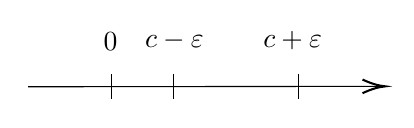
\begin{tikzpicture}[x=0.75pt,y=0.75pt,yscale=-1,xscale=1]
			%uncomment if require: \path (0,300); %set diagram left start at 0, and has height of 300
			
			%Straight Lines [id:da351590380041958] 
			\draw    (270,110.6) -- (440,110.4) ;
			\draw [shift={(442,110.4)}, rotate = 179.93] [color={rgb, 255:red, 0; green, 0; blue, 0 }  ][line width=0.75]    (10.93,-3.29) .. controls (6.95,-1.4) and (3.31,-0.3) .. (0,0) .. controls (3.31,0.3) and (6.95,1.4) .. (10.93,3.29)   ;
			%Straight Lines [id:da6689641897087604] 
			\draw    (310,104.6) -- (310,116.6) ;
			%Straight Lines [id:da03212271146730217] 
			\draw    (340,104.6) -- (340,116.6) ;
			%Straight Lines [id:da4012489765266216] 
			\draw    (400,104.6) -- (400,116.6) ;
			
			% Text Node
			\draw (305,83.4) node [anchor=north west][inner sep=0.75pt]    {$0$};
			% Text Node
			\draw (325,82.4) node [anchor=north west][inner sep=0.75pt]    {$c-\varepsilon $};
			% Text Node
			\draw (382,82.4) node [anchor=north west][inner sep=0.75pt]    {$c+\varepsilon $};
		\end{tikzpicture}
	\end{center}
	Per definizione di estremo inferiore, esiste $g \in \Gamma$ tale che
	\[ \underset{t \in [0,1]}{\max}\; I[g(t)] \le c +\delta, \]
	ossia, per ogni $t \in [0,1]$, $g(t) \in A_{c+\delta}$. Poniamo $\hat{g} = \eta \circ g$. Chiaramente $\hat{g} \in C([0,1];X)$. Inoltre, $\hat{g}(0) = \eta(0) = 0$ e $\hat{g}(1)= \eta(v) = v$, quindi $\hat{g} \in \Gamma$. Siccome $g(t) \in A_{c+\delta}$, allora $\hat{g}(t) \in A_{c-\delta}$, quindi 
	\[ \underset{t \in [0,1]}{\max}\; I[\hat{g}(t)] \le c -\delta, \]
	da cui $c \le c-\delta$, assurdo.
\end{proof}
\begin{osservazione}
	Pensiamo al caso $X = \R^2$. In questa situazione il grafico di $I$ è un "lenzuolo" sopra il piano $xy$. Sappiamo che l'origine è circondato da punti ad altezza $a$ e che esiste un punto che sta sotto il piano $xy$. Se partendo dall'origine volessi raggiungere tale punto dovrò necessariamente "salire" e poi "scendere": nel percorrere questo passo, attraverserò un punto critico per $I$.
\end{osservazione}


Il lettore interessato può approfondire altri aspetti legati al Calcolo delle Variazioni cominciando da
\textsc{B. Dacorogna}, \emph{Introduction to the Calculus of Variations}, Imperial College Press, London, 2014. Un altro testo, più recente, può essere \textsc{L. Brasco}, \emph{Handbook of Calculus of Variations for Absolute Beginners}, Springer, Cham, 2025.